\documentclass{article}
\usepackage[margin=2cm]{geometry}
\usepackage{hyperref}
\usepackage{graphicx}
\usepackage{amsmath}
\usepackage{amsfonts}
\usepackage{tikz}
\title{Multilayer Perceptrons for Dynamic Branch Prediction as a Function of Global History}
\author{Andrew Bruce \\ \href{mailto:acbruce@ucsc.edu}{acbruce@ucsc.edu}
  \and Gowrav BG \\ \href{mailto:gbukkapa@ucsc.edu}{gbukkapa@ucsc.edu} }

\begin{document}
\maketitle

\begin{abstract}
  \indent More accurate branch prediction means the CPU pipeline will require less misprediction flush, increasing the number of instructions per cycle. In this paper we fit perceptrons on the global history, allowing the perceptrons to be dynamically updated and adapt to changing workloads.
\end{abstract}
\section{Implementation}
We created a table of $P \in \mathbb{N}$ perceptrons. When a conditional branch instruction is encountered with virtual memory address $A \in \mathbb{N}$, it uses perceptron index $A \mod P$. We implemented a more complex hashing algorithm, but it did not affect performance so we did not continue down this route.
\section*{Single layer perceptron}
We first tried single layer perceptrons. Given $N \in \mathbb{N}$ history bits, the perceptron at index $A \mod P$ will predict if the conditional branch is taken or not taken based on the global history bits $H \in \{ -1, 1 \}^N$.
\subsection*{Inference algorithm}
Each perceptron has weights $W \in \mathbb{Z}^N$ and a bias $b \in \mathbb{Z}$. The prediction of taken or not taken will be $y \in \{-1, 1\}$, where $-1$ and $1$ represent not taken or taken respectively.\\
\begin{center}
  $y = \text{sign}(b + \sum_{i=1}^N W_i H_i)$
\end{center}
\subsection*{Training algorithm}
In the case of an incorrect prediction, with the correct prediction of $y_{correct} \in \{-1, 1\}$, the weights and biased are updates according to the following algorithm\cite{article}.
\begin{center}
  $W_{t+1, i} = W_{t, i} + y_{correct}(H_i)$\\
  $b_{t+1} = b_t + y_{correct}$
\end{center}
\section*{Double layer perceptron}
A double layer perceptron with $K$ intermediate values will have $W_k \in \mathbb{R}^N$, and biases $b_k \in \mathbb{R}$ where $k \in \{ 1 \cdots K\}$. The second layer will have weights $X \in \mathbb{R}^K$ and bias $c \in \mathbb{R}$.
\subsection*{Inference algorithm}
The inference algorithm is similar, but to we need a non-linear activation function $\sigma$ to prevent the inference from becoming a simple linear transformation with a bias which is equivelent to a single layer perceptron. The inference first calculates the intermediate values $V_k \in \mathbb{R}, k \in \{ 1 \dots K \}$.
\begin{center}
  $V_k = \sigma(b_k + \sum_{i = 1}^N W_{k, i}H_i)$\\
  $y = \text{sigm}(c + \sum{i = 1}^K X_iV_i)$
\end{center}
\subsection*{Training algorithm}
For a double layer perceptron we designed an update algorithm for each incorrect prediction. It is equivelent to gradient descent with a learning rate of 1 in a modern feed forward network.
\begin{center}
  $X_{t+1, k} = X_{t, k} + y_{correct}(V_k)$\\
  $c_{t+1} = b_t + y_{correct}$\\
  $W_{t+1, k, i} = W_{t, k, i} + \frac{d\sigma(V_k)}{dV_k} X_{t, k} H_i$\\
  $b_{t+1, k} = b_{t, k} + \frac{d\sigma(V_k)}{dV_k} X_{t, k}$
\end{center}
In our implementation we used the sigmoid activation function: $\sigma(x) = \dfrac{1}{1 + e^{-x}}$, and $\dfrac{d\sigma(x)}{dx} = \sigma(x) (1 - \sigma(x))$.
\section*{Results}
\subsection*{Single Layer}
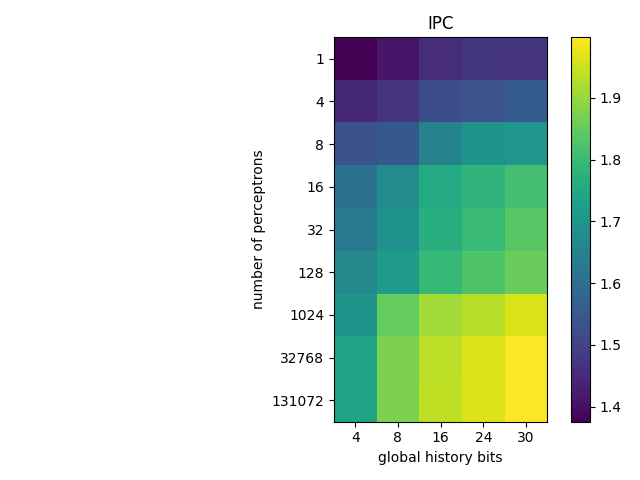
\includegraphics[width=0.5\textwidth]{./cse220data/data_1_layer/matrix_ipc_all.png}
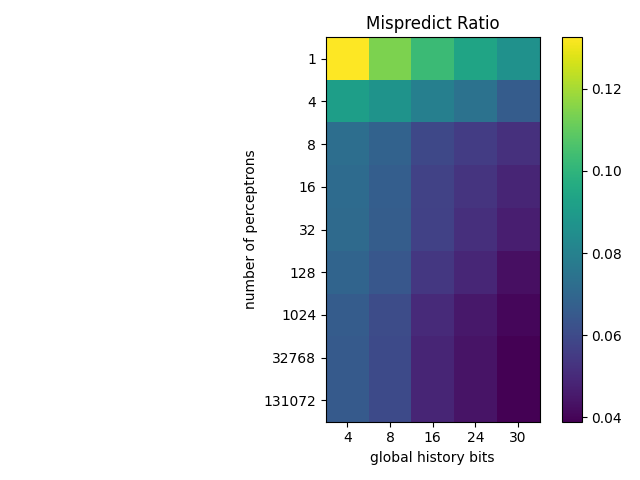
\includegraphics[width=0.5\textwidth]{./cse220data/data_1_layer/matrix_mispred_all.png}
There is a clear correlated decrease in the misprediction ratio when the size of the perceptron table and the number of global history bits increases. With just a single perceptron and only 4 global history bits, the branch predictor was able have a miss rate of only 0.128.\\
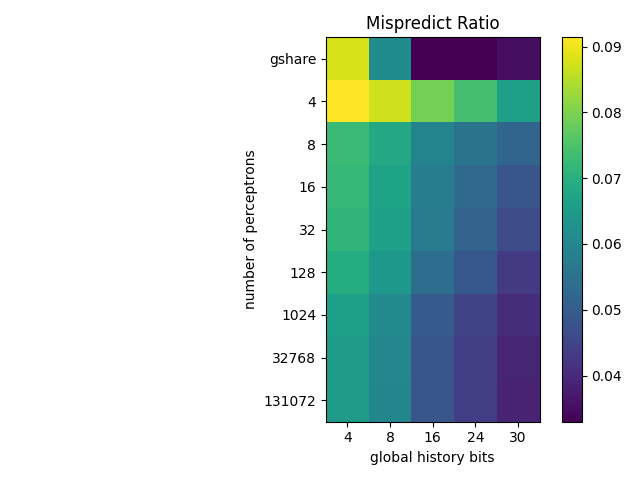
\includegraphics[width=0.5\textwidth]{./cse220data/data_1_layer/matrix_mispred_gshare.png}
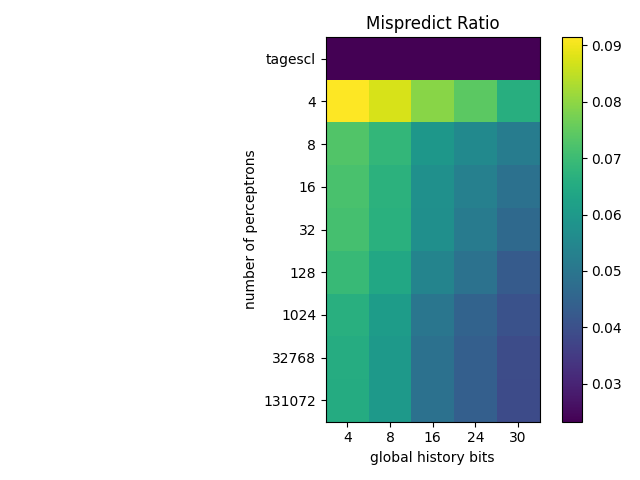
\includegraphics[width=0.5\textwidth]{./cse220data/data_1_layer/matrix_mispred_tagescl.png}
When compared to gshare, the single layer perceptrons perform better with a low amount of history bits, but gshare performs better with history bits greater than 16. This result is probably because it is impossible for a single layer perceptron to learn non-linearely seperable data allowing gshare to perform better when a large amount of branches are inseperable. Another possibility is the chosen subset of workloads favor gshare due to branches changing in patterns that the perceptrons dynamic adaption fails to adapt to fast enough.\\
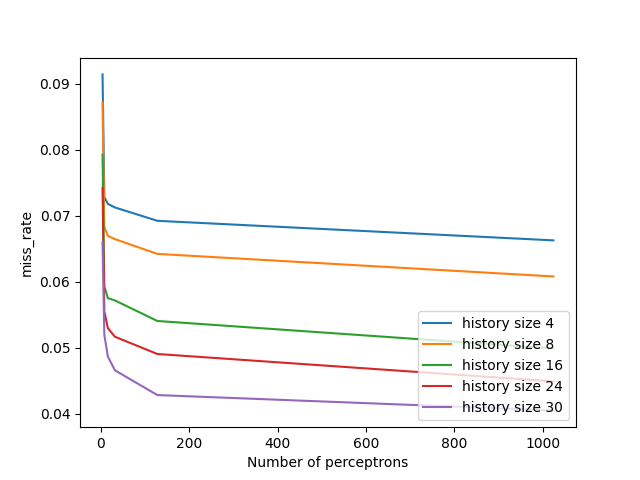
\includegraphics[width=0.5\textwidth]{./cse220data/data_1_layer/x_num_perceptrons_no_last_2.png}
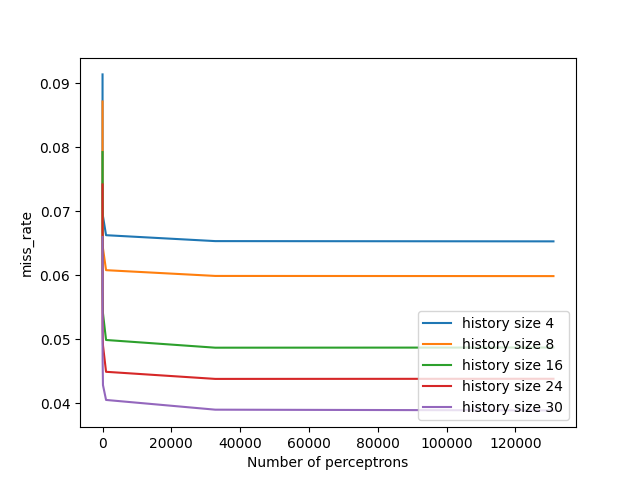
\includegraphics[width=0.5\textwidth]{./cse220data/data_1_layer/x_num_perceptrons_all.png}
We found diminishing returns after 32768 perceptrons. We theorize the plateu is theorized to be due to the collision rate between conditional branch instructions in the perceptron table to drop between a sufficient level that adding more perceptrns doesn't prevent many additional collisions. Assuming the address of conditional branch instructions are uniformly distributed, the chance of two instructions colliding is $\dfrac{1}{N}$, which asymptomatically approaches zero as $N$ increases, explaining the diminishing returns.\\
\begin{center}
  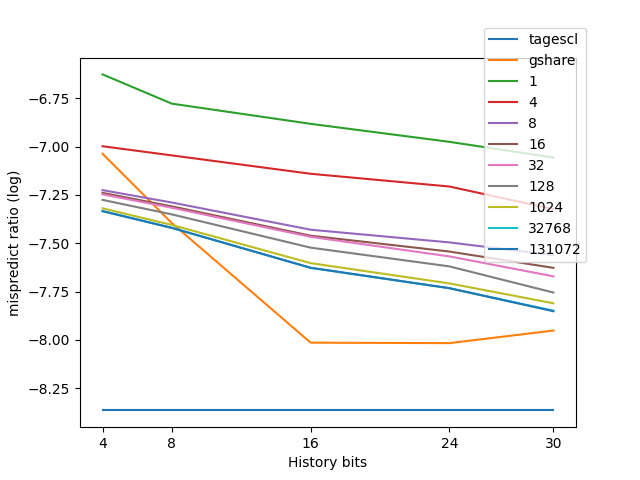
\includegraphics[width=0.5\textwidth]{./cse220data/data_1_layer/x_hist.png}
\end{center}
This graph shows how gshare surpasses all of the single layer perceptron configurations as the number global history bits increases.
\subsection*{Double Layer}
Our double layer perceptrons had five intermediate values.
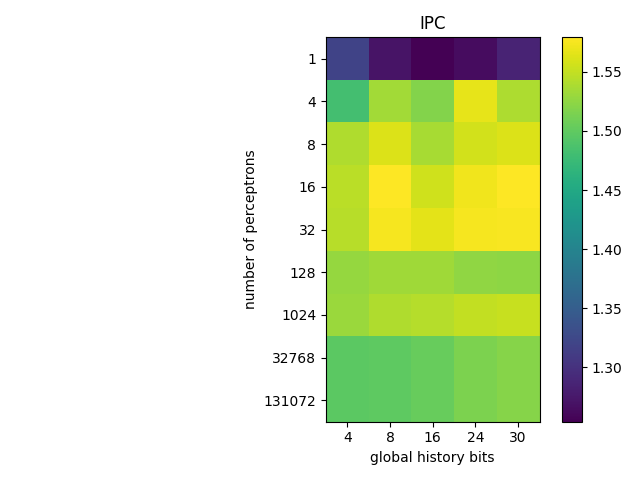
\includegraphics[width=0.5\textwidth]{./cse220data/data_2_layer/matrix_ipc_all.png}
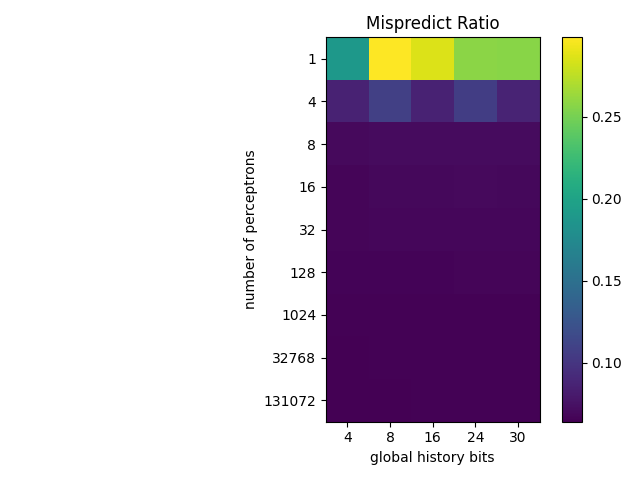
\includegraphics[width=0.5\textwidth]{./cse220data/data_2_layer/matrix_mispred_all.png}
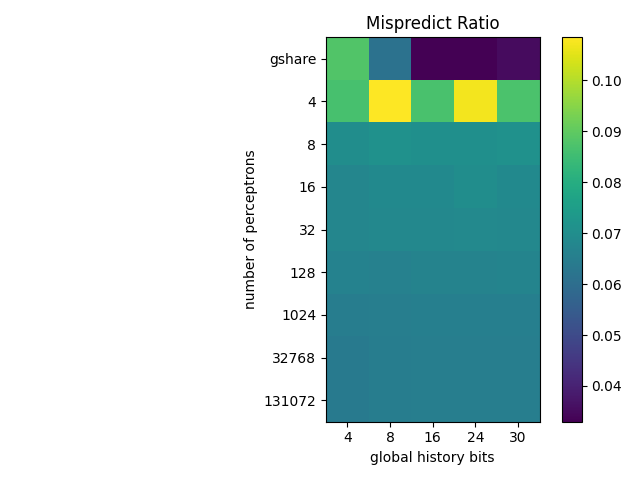
\includegraphics[width=0.5\textwidth]{./cse220data/data_2_layer/matrix_mispred_gshare.png}
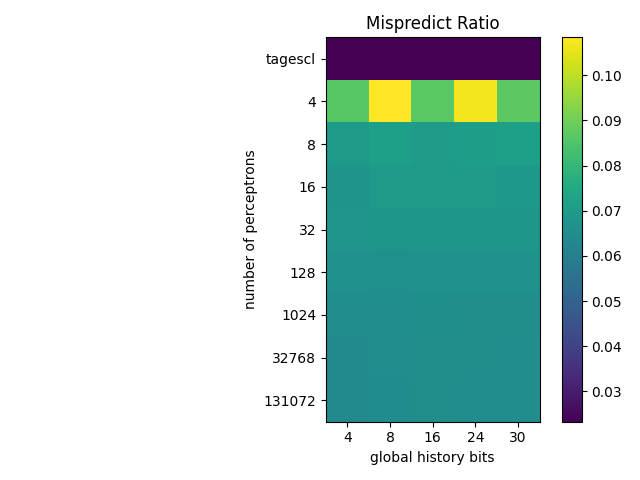
\includegraphics[width=0.5\textwidth]{./cse220data/data_2_layer/matrix_mispred_tagescl.png}
The double layer perceptron seems to fit the data significanly worse than a single layer perceptron. We suspect this is due to higher variance causing overfitting because each perceptron has greater number of parameters. Each double layer has greater than five times the parameters of a single layer perceptron, allowing for higher variance over the datasets. Possible solutions could be decreasing the number of intermediate values to decrease the number of parameters, and to decrease the learning rate in the training algorithm.
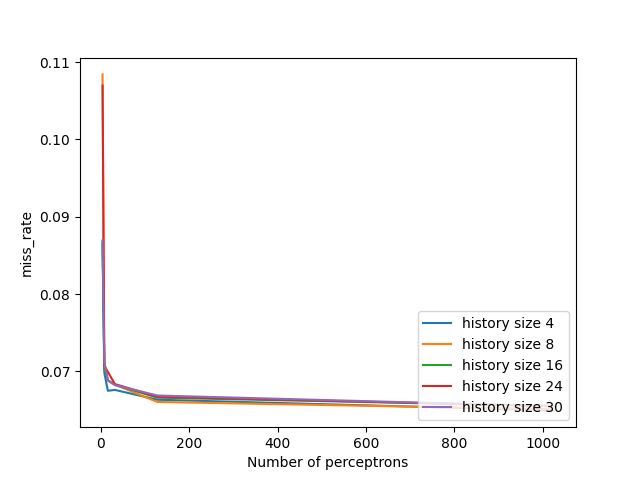
\includegraphics[width=0.5\textwidth]{./cse220data/data_2_layer/x_num_perceptrons_no_last_2.png}
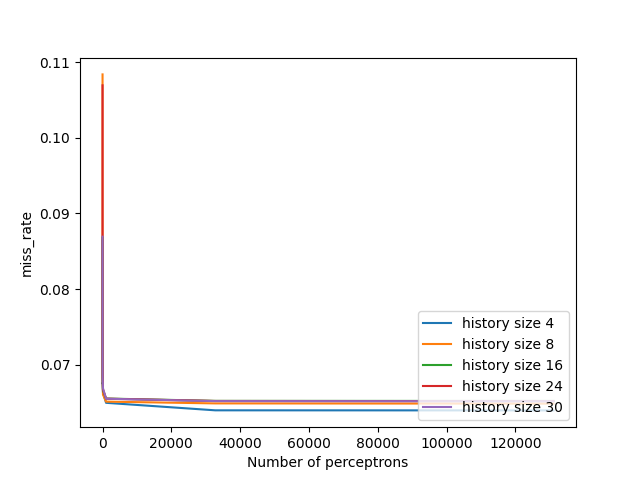
\includegraphics[width=0.5\textwidth]{./cse220data/data_2_layer/x_num_perceptrons_all.png}
Increasing the number of perceptrons still lowers the misprediction rate. This decrease is probably do to decrease variance since less collisions mean a smaller total possible samples that the model must generaize over.
\begin{center}
  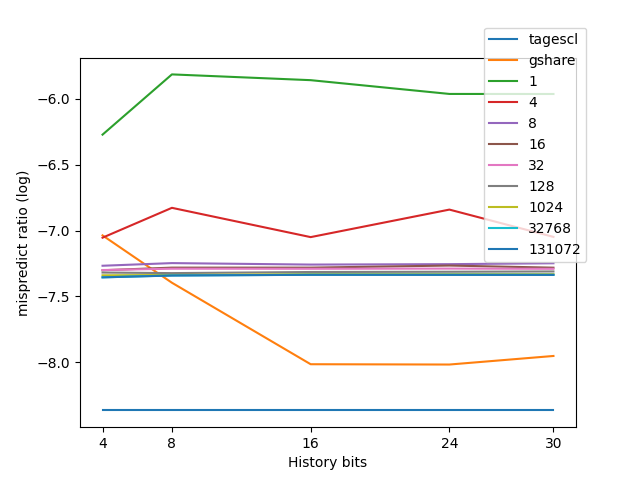
\includegraphics[width=0.5\textwidth]{./cse220data/data_2_layer/x_hist.png}
\end{center}
Changing the history size had little effect on the the mispredition ratio. One theory is the increased variance already maxes out on just a four history bits, meaning increase history bits provide no extra information to the perceptron can correlate.

\bibliographystyle{abbrv}
\bibliography{refs}

\end{document}
